% !TEX root = epifanov_solid_state_physics.tex
%!TEX TS-program = pdflatex
%!TEX encoding = UTF-8 Unicode


\chapter[Contact Phenomena]{Contact Phenomena}\label{chap:8}
% \chaptermark{The Band Theory of Solids}

\section{Work function}\label{sec:73}

\textbf{The work function concept.} The positive ions that make up the metal lattice establish in it an electric field with a positive potential that changes periodically along a straight line passing through the lattice sites [\fig{8_1}(a)]. As a rough approximation, this variation may be neglected and the potential be considered constant and equal to $V_0$ at every point of the metal. A free electron has a negative potential energy $U_0=-qV_0$ in this field ($q$ is the electron charge).

Figure \ref{fig:8_1}(b) depicts the change in the potential energy of the electron as it passes from the vacuum into the metal: in vacuum $U=0$, in the metal $U=U_0=-qV_0$. Although such a change has the nature of a jump, it takes place over a distance $\delta$ equal approximately to the lattice parameter. It may be seen from \fig{8_1}(b) that the metal is a potential trough for the electron and that work should be performed to get the electron out of it. This work is termed the \textit{work function}.

Should the electrons have no kinetic energy, the work needed to liberate them would be equal to the depth of the potential trough $U_0$. However, electrons possess kinetic energy of translational motion, even at absolute zero, since they occupy all the lower energy levels of the potential trough up to the Fermi level $\mu$. Therefore, the energy needed to make them leave the metal is less than $U_0$. The least work must be performed to liberate the electrons occupying levels close to the Fermi level. It is equal to the separation $\chi$ of the Fermi level from the zero level and the term for it is \textit{thermodynamic work function}.

\begin{figure}[t]
	\begin{center}
		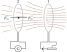
\includegraphics[scale=1]{figures/ch_08/fig_8_1.pdf}
		\caption[]{Metal as a potential through: (a)---internal potential of metal; (b)---potential energy of electron in metal.}
		\label{fig:8_1}
	\end{center}
	\vspace{-0.8cm}
\end{figure}

The problem of estimating the electron work function of a semiconductor is somewhat more complicated. As may be seen from \fig{8_2} the electrons may leave the semiconductor from the levels of the conduction band at the expense of work $\chi_0$, from the impurity levels at the expense of work $\chi_1$ and from the levels of the valence band at the
expense of work $\chi_2$ and $\chi_3$. The least work $\chi_0$ is required to liberate the electrons from the conduction band. However, emission of only the conduction electrons would upset the equilibrium of the electron gas, to reestablish which the electrons should go over to the conduction band from the impurity levels and from the valence band. Such transitions require work to be performed and, in adiabatic conditions, this work is performed at the expense of the internal energy of the crystal, that is, as the state of thermal equilibrium is restored the crystal is cooled. If the electrons leave the semiconductor from the valence band, to restore equilibrium some electrons must go over from the conduction band to the valence band, which results in liberation of energy and the crystal being heated. The equilibrium will be maintained and the temperature will remain constant only if the electrons
leave the semiconductor from the levels both below and above the Fermi level in appropriate numbers. Theory shows that to maintain equilibrium the average energy of the electrons leaving the semiconductor should be equal to the Fermi energy, and this is the work function, although there may be no electrons on the Fermi level itself.

The work function is measured in electron volts. The ratio of the work function to the electron charge is the voltage equivalent of the work function. The work function measured in electron volts is numerically equal to its voltage equivalent.

\begin{figure}[t]
	\begin{center}
		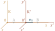
\includegraphics[scale=1]{figures/ch_08/fig_8_2.pdf}
		\caption[]{Electron work function of semiconductor.}
		\label{fig:8_2}
	\end{center}
	\vspace{-0.8cm}
\end{figure}

\textbf{Effect of adsorbed layers on work function.} Molecular layers adsorbed by the surface of the solid, in particular monomolecular layers, greatly affect the work function. Figure \ref{fig:8_3}(a) shows a monatomic caesium layer on the surface of tungsten. Caesium is an alkali metal. Its outer valence electron is bonded to the nucleus much more weakly than the valence electrons of the tungsten atom. Therefore, in the process of adsorption caesium donates its valence electron to tungsten and turns into a positively charged ion inducing a negative change of equal magnitude in the metal's surface layer. When tungsten is covered by a monatomic caesium layer, an electric double layer is built up at the surface with its outer side charged positively. The potential difference in this double layer aids electron emission out of tungsten. Therefore, the electron work function, as determined from experiment, drops in the presence of the caesium layer from \SI{4.52}{\electronvolt} for pure tungsten to \SI{1.36}{\electronvolt}. The same is the effect of monatomic layers of other electropositive metals: barium, cerium, thorium, etc.

\begin{figure}[h]
	\begin{center}
		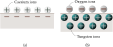
\includegraphics[scale=0.95]{figures/ch_08/fig_8_3.pdf}
		\caption[]{Formation of electric double layer in the course of adsorption of caesium (a) and of oxygen (b) on tungsten surface.}
		\label{fig:8_3}
	\end{center}
	\vspace{-0.8cm}
\end{figure}

The reduction of the work function by the adsorption of electropositive metals is widely used for manufacturing vacuum tube cathodes, photocathodes, etc.

Quite different is the effect of oxygen adsorbed on the metal's surface. The valence electrons in the oxygen atom are bonded much more strongly than in metals. Therefore, in the process of adsorption
the oxygen atom instead of donating electrons, accepts two electrons from the metal and turns it into a negatively charged ion. As a result, the outer side of the electric double layer becomes negatively
charged [\fig{8_3}(b)] and the resulting electric field prevents the electrons from leaving the metal, thereby, increasing the work function.

\section{Contact of two metals}\label{sec:74}

\textbf{Contact potential difference.} Consider the process which takes place when two metals [\fig{8_4}(a)] whose energy diagrams are shown in [\fig{8_4}(b)] are brought together.

The electron gas in the individual metals $1$ and $2$ is characterized by the respective chemical potentials $\mu_1$ and $\mu_2$, the thermodynamic work functions being $\chi_1$ and $\chi_2$. Let us bring the metals closer together, to within such a distance $d$, that an effective electron exchange by means of thermionic emission or by direct transition from one metal to another, is possible. At the initial moment after the contact has been established, there will be no equilibrium between the electron gas in the first and second metals since the chemical potential (the Fermi level) $\mu_2$ is above $\mu_1$. The difference in the Fermi levels, $\mu_2-\mu_1$, results in the prevailing transition of the electrons from the second metal to the first one, in the course of which the first metal is charged negatively and the second positively. The appearance of the charges causes a shift in the energy levels of the metals: all the levels in the negatively charged metal $1$ rise and in the positively charged metal $2$ sink as compared with their positions in uncharged metals. This may easily be understood from the following simple considerations. To move an electron from, for instance, the zero level of an uncharged metal to the zero level of a metal charged negatively to a potential $V_1$, work should be performed numerically equal to $qV_1$. This work is transformed into the potential energy of the electron. Therefore, the potential energy of an electron occupying the zero level of the negatively charged metal will be higher, by the amount $qV_1$, than the potential energy of an electron occupying the zero level of the uncharged metal. The zero level of a positively charged metal sinks below the zero level of an uncharged metal, the reason for this being the same. A similar shift occurs in the position of other energy levels of the metals $1$ and $2$ including that of the Fermi level.

\begin{figure}[t]
	\begin{center}
		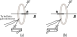
\includegraphics[scale=1]{figures/ch_08/fig_8_4.pdf}
		\caption[]{Origin of contact potential difference between n-type conductors.}
		\label{fig:8_4}
	\end{center}
	\vspace{-0.8cm}
\end{figure}

As soon as the continuously rising chemical potential of the metal $1$ ($\mu_1$) and the continuously sinking chemical potential of the metal
$2$ ($\mu_2$) level out [\fig{8_4}(c)], the cause for the predominant flow of the electrons from the first metal to the second disappears, and a dynamic equilibrium is established between the metals, resulting in the corresponding constant potential difference between the zero levels of both metals [\fig{8_4}(c)] equal to
\begin{equation}\label{eq:8_1}
    \ab{V}{c} = \frac{(\chi_1 - \chi_2)}{q}.
\end{equation}

\noindent
This potential difference is termed the \textit{external contact potential difference}. It follows from \eqn{8_1} that it owes its existence to the difference in electron work functions of the contacting metals: the electrons leave the metal with the smaller work function and settle in the metal with the greater work function.

After the chemical potentials have been equalized, the kinetic energy of electrons occupying levels close to the Fermi levels of both metals is not the same: that of electrons in metal $1$ is equal to $\ab{E}{F$1$}$ and that of electrons in metal $2$ to $\ab{E}{F$2$}$ ($\ab{E}{F$2$}>\ab{E}{F$2$}$). When a direct contact is established between the two metals, a predominant diffusion process of the electrons from the second metal to the first sets in, and continues until the so-called \textit{internal contact potential difference}
\begin{equation}\label{eq:8_2}
    \ab{V}{i} = \frac{(\ab{E}{F$2$} - \ab{E}{F$1$})}{q}.
\end{equation}

\noindent
is established.

\textbf{Thickness of the electric double layer at the contact of two metals.} A double layer [\fig{8_5}(a)] is established at the contact of two metals across which the potential changes abruptly by the amount $V_1$ [\fig{8_5}(b)]. Let us estimate the thickness of this layer. Suppose that it is a plane condenser with the distance between the plates equal to the double layer thickness $d$. Denote the charge on each plate by $Q$ and the potential difference by $V_1$. The capacitance of a plane condenser with the plate area of \SI{1}{\metre\squared} and a dielectric with relative
permittivity $\varepsilon=1$ is $C=\varepsilon_0/d$ ($\varepsilon_0$ is the permittivity of free space).
Using the relation $C=Q/V_1$, we can rewrite this formula in the form $Q/V_1=\varepsilon_0/d$. Hence, we obtain
\begin{equation*}
    d = \frac{\varepsilon_0 V_1}{Q}.
\end{equation*}

\begin{figure}[t]
	\begin{center}
		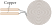
\includegraphics[scale=1]{figures/ch_08/fig_8_5.pdf}
		\caption[]{External ($\ab{V}{c}$) and internal ($\ab{V}{i}$) contact potential differences appearing at the instant two different metals are brought in contact.}
		\label{fig:8_5}
	\end{center}
	\vspace{-0.8cm}
\end{figure}

The thickness of the double layer cannot be less than the lattice parameter $a\approx\SI{3}{\angstrom}$. At $\ab{V}{i}\approx\SI{1}{\electronvolt}$ such a layer can be established if a charge $Q\approx\ab{V}{i}\varepsilon_0/a\approx\SI{3e-2}{\coulomb}$ is transported from every square metre of the contact surface of the first metal to the second. This corresponds to $\Delta{n}=Q/q\approx\SI{2e17}{\per\metre\squared}$ electrons. There are approximately \num{e19} atoms on every square metre of a metal. If we assume that each of them donates to the electron gas one valence electron, we will obtain for the surface density of the electron gas the value $\ab{n}{s}\approx\SI{e19}{\per\metre\squared}$.
Comparing $\Delta{n}$ with $\ab{n}{s}$, we see that even for the narrowest possible double layer ($a\approx\SI{3}{\angstrom}$) only two percent of free electrons need be transported from the contact surface of one metal to another.

Because of a small change in the electron concentration in the contact layer, and because of the small thickness of this layer in comparison with the electron mean free path, the conductivity of the layer cannot be much less than that of the bulk metal. The current passes through the contact of two metals just as easily as through the metals themselves.

\section{The metal-semiconductor contact}\label{sec:75}

\textbf{Barrier layer.} Consider a metal-semiconductor contact. Suppose that a metal with its work function equal to $\ab{\chi}{m}$ is brought in contact with an n-type semiconductor whose work function is $\ab{\chi}{s}$ (\fig{8_6}).

If $\ab{\chi}{m}>\ab{\chi}{s}$ the electrons will flow out of the semiconductor into the metal until the chemical potentials $\ab{\mu}{m}$ and $\ab{\mu}{s}$ are equalized and a state of equilibrium is established. A contact potential difference $\ab{V}{c}$ will be established between the metal and the semiconductor whose order of magnitude will be the same as that in the metal-metal
contact (several volts). To establish such a contact potential difference approximately the same number of electrons should be transported from the semiconductor to the metal as in the case of the contact of two metals. For a lattice parameter of the semiconductor $a\approx\SI{5}{\angstrom}$ (germanium) and an electron gas concentration in it
$n\approx\SI{e21}{\per\metre\cubed}$, there will be $\ab{n}{s}\approx\num{e14}$ electrons on \SI{1}{\metre\squared} of the semiconductor's surface. Therefore, the transport of $\Delta{n}\approx\num{e17}$ electrons entails the ``depletion'' of about \num{e3} atomic layers of the semiconductor.

\begin{figure}[t]
	\begin{center}
		
\includegraphics[scale=1]{figures/ch_08/fig_8_6.pdf}
		\caption[]{Formation of barrier layer in metal-semiconductor contact.}
		\label{fig:8_6}
	\end{center}
	\vspace{-0.8cm}
\end{figure}

Hence, the equalization of the chemical potentials of a metal and a semiconductor in contact with one another necessarily involves the transport of electrons to the metal surface from a boundary layer of appreciable width $d$ of the semiconductor (\fig{8_6}). The ionized impurity atoms remaining in this layer establish a static positive space charge. Since there are practically no free charge carriers inside this layer and since its width greatly exceeds the electron mean free path, its specific resistance is very great and because of that it is termed \textit{barrier layer}.

\textbf{Effect of contact field on semiconductor energy levels.} The contact potential difference $\ab{V}{c}$ between the metal and the semiconductor is built up over the entire width $d$ of the barrier layer (\fig{8_6}). Assuming that $a\approx\SI{5}{\angstrom}$, we obtain for the number of depleted atomic layers $\Delta{N}\approx\num{e3}$ and for the thickness of the barrier layer $d\approx\SI{5e3}{\angstrom}\approx\SI{e-7}{\metre}$.
For $\ab{V}{c}\approx\SI{1}{\volt}$, the field intensity will be $\ab{\mathcal{E}}{c}\approx\ab{V}{c}/d\approx\SI{2e6}{\volt\per\metre}$. This is at least three orders of magnitude less than the intensity of the internal crystal field, which is responsible for the energy band pattern of the semiconductor. Therefore, the contact field cannot appreciably affect the band spectrum (the forbidden band width, the impurity ionization energy, etc.). Its action is limited to the deflection of the semiconductor's energy bands. Let us dwell on this.

\begin{figure}[t]
	\begin{center}
		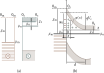
\includegraphics[scale=1]{figures/ch_08/fig_8_7.pdf}
		\caption[]{Effect of contact field on semiconductor's energy levels: (a)---band patterns of metal M and semiconductor S; (b)---deflection of semiconductor's energy bands by contact field.}
		\label{fig:8_7}
	\end{center}
	\vspace{-0.8cm}
\end{figure}

Figure \ref{fig:8_7}(a) shows the energy band diagrams of the metal M and the semiconductor S before they have been brought in contact. When contact has been achieved and equilibrium has been established, a positive space charge throughout the barrier layer width $d$ is built up [\fig{8_7}(b)]. In the absence of the contact field, the energy levels in the metal and in the semiconductor are represented by horizontal straight lines. This expresses the fact that the energy of an electron occupying this level, for instance, the lower level of the conduction band, is the same everywhere in the semiconductor and does not depend on the position of the electrons. In the presence of a contact potential difference the picture is changed: inside the layer in which the contact field is concentrated, a force acts on the electron pushing it out of the layer. To overcome this force, work should be performed, this work being equal to the potential energy of the electron in the contact field. Therefore, as the electron moves inside the space charge layer its potential energy $\varphi(x)$ increases reaching its maximum $\varphi_0=q\ab{V}{c}$ at the semiconductor's surface. Quantum mechanical calculations lead to the conclusion that the application of an external field to the semiconductor results in an inclination of its energy bands in relation to the horizontal Fermi level. The contact field acts in the same way causing a deflection of the energy bands. The quantity $\varphi_0$ is termed the \textit{equilibrium potential barrier} for electrons
going over from the semiconductor to the metal.

To estimate the function $\varphi(x)$ we apply the Poisson equation known from electrostatics. This equation relates the field potential $V(x)$ to the density $\rho(x)$ of the static space charge responsible for this field. The equation is of the form
\begin{equation}\label{eq:8_3}
    \diffsec{V}{x} = - \frac{\rho(x)}{\varepsilon_0 \varepsilon}
\end{equation}

\noindent
where $\varepsilon$ is the relative permittivity of the semiconductor.

It is expedient to go over from the potential $V(x)$ to the potential energy of the electron $\varphi(x)= -qV(x)$ and to write the Poisson equation for $\varphi(x)$ as
\begin{equation}\label{eq:8_4}
    \diffsec{\varphi}{x} = \frac{q}{\varepsilon_0 \varepsilon} \rho(x).
\end{equation}

In calculating the space charge density $\rho(x)$ we shall assume all the donor atoms $\ab{N}{d}$ to be ionized and their electrons to be transferred to the metal. Then $\rho(x)=q\ab{N}{d}$. Substituting this into the Poisson equation, we obtain
\begin{equation}\label{eq:8_5}
    \diffsec{\varphi}{x} = \frac{q^2}{\varepsilon_0 \varepsilon} \ab{N}{d}.
\end{equation}

If we assume that there is no contact field at a distance $x\gg d$ inside the semiconductor, we will be able to write the boundary conditions for this equation in the form
\begin{equation}\label{eq:8_6}
    \varphi(d) = 0,\quad \bracket{\diff{\varphi(x)}{x}}_{x=d} = 0.
\end{equation}

Solution of \eqn{8_5} with the boundary conditions \eqref{eq:8_6} yields:
\begin{equation}\label{eq:8_7}
    \varphi(x) = \frac{q^2 \ab{N}{d}}{2\varepsilon_0 \varepsilon} (d - x)^2.
\end{equation}

\noindent
It follows from \eqn{8_7} that the potential of the contact field diminishes parabolically with the increase in $x$ in the semiconductor.

For $x=0$, we find that $\varphi_0=\ab{\chi}{m}-\ab{\chi}{s}$. Substituting this into \eqn{8_7}, we obtain the width of the barrier layer:
\begin{equation}\label{eq:8_8}
    d = \parenthesis{\frac{2 \varepsilon_0 \varepsilon \varphi_0}{q^2 \ab{N}{d}}}^{1/2} = \parenthesis{\frac{2 \varepsilon_0 \varepsilon \ab{V}{c}}{q \ab{n}{n$0$}}}^{1/2}
\end{equation}

\noindent
where $\ab{n}{n$0$}=\ab{N}{d}$ is the concentration of electrons (majority carriers) in the n-type semiconductor.

It follows from \eqn{8_8} that the thickness of the barrier layer $d$ increases with the contact potential difference $\ab{V}{c}$ determined by the difference in work functions and decreases with the concentration of majority carriers in the semiconductor. Table \ref{table:8_1} shows the values of $d$ calculated with the aid of \eqn{8_8} assuming that $\ab{V}{c}=\SI{1}{\volt}$ and $\varepsilon=10$.

\begin{table}[!b]
	\renewcommand{\arraystretch}{1.2}
	\caption{}
	\vspace{-0.6cm}
	\label{table:8_1}
	\begin{center}\resizebox{0.3\linewidth}{!}{
			\begin{tabular}{cc}
				\toprule[1pt]
                $\ab{n}{n$0$}$ $\parenthesis{\si{\per\metre\squared}}$ & $d$ (\si{\metre})\\
                \midrule[0.5pt]\midrule[0.5pt]
                \num{e24} & \num{3e-7}\\
                \num{e22} & \num{3e-6}\\
                \num{e20} & \num{3e-5}\\
				\bottomrule[1pt]
			\end{tabular}
	}\end{center}
\end{table}

It follows from the table that for the electron gas concentrations typical of semiconductors (\SIrange{e20}{e24}{\per\metre\cubed}), the thickness of the surface layer containing practically no free carriers may attain values from one to three orders of magnitude greater than the electron mean free path. This is the reason why the resistance of the barrier layer is enormous.

If the work function of an n-type semiconductor exceeds that of a metal, $\ab{\chi}{s}>\ab{chi}{m}$, the electrons shall be transported from the metal to the semiconductor setting up a negative charge in its contact layer (\fig{8_8}). In this case, the energy of the electron $\varphi(x)$ as it approaches the surface does not increase but, on the contrary, decreases with the result that the bands are deflected in the opposite direction. This leads to an increase in the free charge carrier concentration inside the contact layer of the semiconductor and to a consequent increase in its conductivity. For this reason such a layer is termed \textit{antibarrier}.

\begin{figure}[t]
	\begin{center}
		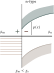
\includegraphics[scale=1]{figures/ch_08/fig_8_8.pdf}
		\caption[]{Formation of antibarrier layer in metal-semiconductor contact.}
		\label{fig:8_8}
	\end{center}
	\vspace{-0.8cm}
\end{figure}

\textbf{Rectification at a metal-semiconductor contact.} A remarkable feature of the barrier layer is a drastic dependence of its resistance on the direction of external voltage applied to the contact. This dependence is so strong that it results in practically a unidirectional conductivity of the contact: a current passes easily through the contact in the forward direction and much worse in the reverse direction. This is the essence of the rectifying property of a metal-semiconductor contact.
Let us discuss this point in detail.

Figure \ref{fig:8_9}(a) shows the energy band pattern of an n-type metalsemiconductor contact in the state of equilibrium. The potential barrier for the electrons going over from the metal to the
semiconductor, is equal to the difference in work functions $\ab{\chi}{m}-\ab{chi}{s}$: for the electrons passing from the semiconductor to
the metal it is $\varphi_0=q\ab{V}{c}$. Denote the electron flux from the metal to the semiconductor by $\ab{n}{m.s}^0$ and the flux from the semiconductor
to the metal by $\ab{n}{s.m}^0$. The corresponding current densities flowing through the contact are
$\ab{i}{s.m}$ and $\ab{i}{m.s}$. Since in the state of equilibrium the total current flowing through the contact is zero, it follows that $\ab{i}{s.m}=\ab{i}{m.s}$. Denote the current density corresponding to the equilibrium currents $\ab{i}{s.m}^0$ and $\ab{i}{m.s}^0$ by $\ab{i}{eq}$:
\begin{equation}\label{eq:8_9}
    \ab{i}{s.m}^0 = \ab{i}{m.s}^0 = \ab{i}{eq}.
\end{equation}

\begin{figure}[t]
	\begin{center}
		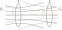
\includegraphics[scale=1]{figures/ch_08/fig_8_9.pdf}
		\caption[]{Rectification in metal-semiconductor contact: (a)---equilibrium state of contact; (b)---external voltage applied in reverse direction; (c)---external voltage applied in forward direction.}
		\label{fig:8_9}
	\end{center}
	\vspace{-0.8cm}
\end{figure}

Apply an external potential difference $V$ to the contact in the direction of the contact potential difference $\ab{V}{c}$ imparting a positive charge to the semiconductor with respect to the metal [\fig{8_9}(b)]; such direction of $V$ is termed \textit{reverse}. The resistance of the barrier layer is usually some orders of magnitude greater than the resistance of the other parts of the circuit and, because of that, practically the entire applied voltage is built up across the barrier layer. The energy levels in the positively charged semiconductor are deflected downwards by $qV$ from their initial positions. The same will be the displacement of the Fermi level $\ab{\mu}{n}$. The deflection takes place along the entire barrier layer thickness d across which the potential rises by $V$. The bottom of the conduction band $\ab{E}{c}$ and the top of the valence band $\ab{E}{v}$ in \fig{8_9}(b) have been drawn so as to take account of the new position of the Fermi level. It may be seen from this drawing that the external voltage $V$ applied in the reverse direction raises the potential barrier for the electrons going over from the semiconductor to the metal to
\begin{equation}\label{eq:8_10}
    \varphi(0) = \varphi_0 + qV.
\end{equation}

\noindent
According to \eqn{8_8} the thickness of this barrier layer will be
\begin{equation}\label{eq:8_11}
    d = \bracket{\frac{2 \varepsilon_0 \varepsilon (\ab{V}{c} + V)}{q \ab{n}{n$0$}}}^{1/2}.
\end{equation}

Hence, the external field applied to the contact in the reverse direction raises the potential barrier for the electrons flowing from the semiconductor to the metal and increases the barrier layer width.

The picture will be different if a forward voltage is applied to the contact [\fig{8_9}(c)]. In this case, all the levels of the negatively charged semiconductor including the Fermi level $\ab{\mu}{n}$ are deflected upwards by the amount $qV$, lowering the potential barrier for the electrons flowing from the semiconductor to the metal by the amount $qV$. The barrier height becomes
\begin{equation}\label{eq:8_12}
    \varphi(0) = \varphi_0 - qV.
\end{equation}

The width of the space charge layer decreases accordingly and becomes equal to
\begin{equation}\label{eq:8_13}
    d = \bracket{\frac{2 \varepsilon_0 \varepsilon (\ab{V}{c} - V)}{q \ab{n}{n$0$}}}^{1/2}.
\end{equation}

The change in the potential barrier height disturbs the equilibrium between the electron fluxes flowing through the contact in both directions. When the external voltage $V$ is applied to the contact in
the reverse direction, the current density $\ab{i}{m.s}$, corresponding to the electron flux $\ab{n}{s.m}$ decreases $e^{qV/(\ab{k}{B}T)}$ times, since according to the Boltzmann law the number of electrons flowing from the semiconductor to the metal capable of surmounting the barrier $\varphi_0+qV$ is $e^{qV/(\ab{k}{B}T)}$ times less than the number flowing through the equilibrium barrier $\varphi_0$, that is, $\ab{n}{s.m}=\ab{n}{s.m}^0\,e^{-qV/(\ab{k}{B}T)}$.
Therefore, the current $\ab{i}{m.s}$ becomes equal to
\begin{equation*}
    \ab{i}{m.s} = \ab{i}{eq}\, e^{-qV/(\ab{k}{B}T)}.
\end{equation*}

The current density $\ab{i}{s.m}$, corresponding to the electron flux $\ab{n}{m.s}$, will remain equal to $\ab{i}{eq}$, since the external field does not change the height of the barrier for electrons flowing from the metal to the semiconductor: its height remains equal to the difference in work functions, $\ab{\chi}{m}-\ab{\chi}{s}$.

The total current density in the reverse direction is [\fig{8_9}(b)]
\begin{equation}\label{eq:8_14}
    \ab{i}{r} = \ab{i}{eq}\, e^{-qV/(\ab{k}{B}T)} - \ab{i}{eq} = \ab{i}{eq}\, \bracket{e^{-qV/(\ab{k}{B}T)} - 1}.
\end{equation}

\noindent
The current flows from the semiconductor to the metal. As the reverse voltage $V$ is increased, the exponential $e^{-qV/(\ab{k}{B}T)}$ tends rapidly to zero and the reverse current density to its limit value $\ab{i}{eq}$. The current density $\ab{i}{eq}$ is termed \textit{saturation current density} and $\ab{I}{eq}=\ab{i}{eq} S$ saturation current ($S$ is the cross-sectional area of the metal-semiconductor contact).

When a forward external voltage $V$ is applied [\fig{8_9}(c)], the potential barrier for the electrons flowing from the semiconductor to the metal is lowered by the amount $qV$ and, because of that, the current density of those electrons increases $e^{qV/(\ab{k}{B}T)}$ times in comparison with $\ab{i}{eq}$, becoming
\begin{equation*}
    \ab{i}{m.s} = \ab{i}{eq}\, e^{qV/(\ab{k}{B}T)}.
\end{equation*}

The current density $\ab{i}{s.m}$ remains equal to $\ab{i}{eq}$. Therefore, the density of the forward current (from the metal to the semiconductor) will be
\begin{equation}\label{eq:8_15}
    \ab{i}{r} = \ab{i}{m.s} - \ab{i}{s.m} = \ab{i}{eq}\, \bracket{e^{qV/(\ab{k}{B}T)} - 1}
\end{equation}

\noindent
and it grows exponentially with $V$. Combining \eqn{8_14} with \eqref{eq:8_15}, we obtain
\begin{equation}\label{eq:8_16}
    i = \ab{i}{eq}\, \bracket{e^{\pm qV/(\ab{k}{B}T)} - 1}
\end{equation}

\noindent
($V=|V|$ for forward bias and $V=-|V|$ for the reverse).

Formula \eqref{eq:8_16} is the equation of the current-voltage characteristic (CVC) of a rectifying metal-semiconductor contact. Figure \ref{fig:8_10}
depicts the CVC of such a contact.

\begin{figure}[t]
	\begin{center}
		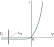
\includegraphics[scale=1]{figures/ch_08/fig_8_10.pdf}
		\caption[]{Current-voltage characteristic of metal-semiconductor contact.}
		\label{fig:8_10}
	\end{center}
	\vspace{-0.8cm}
\end{figure}

The ratio of the forward current to the reverse current for the same absolute value of applied voltage is termed \textit{rectification ratio}. Its value for good rectifying contacts may be as high as tens and even hundreds of thousands.

The potential barrier at the metal-semiconductor interface is often termed \textit{Schottky barrier}. Presently, Schottky barrier diodes with extremely short switching times are being developed. The diodes have switching times as short as \SI{e-11}{\second}. This makes it possible to use them effectively in radioelectronic pulse circuits, in computer and automation circuits where there is a need for high operational speeds, that is, where extremely short and quickly recurring electrical pulses have to be processed.

The nonrectifying (antibarrier) metal-semiconductor contact is used to provide ohmic contacts by means of which the semiconductor device is connected into the electrical circuit.

\section{Contact between two semiconductors of different types of conductivity}\label{sec:76}

The progress in semiconductor electronics is based mainly on the use of contacts of two impurity semiconductors of different conductivity types. Such a contact is termed a \textit{p-n junction}. Let us briefly discuss its properties.

\textbf{Preparation of p-n junctions.} It is impossible to obtain a true p-n junction by means of a mechanical contact of the n- and p-types of semiconductors because the lattice discontinuity at the interface contains more defects than there are impurity atoms on each of the contacting surfaces. Therefore, the p-n junction was successfully prepared only when the art of making it in the form of an internal boundary in the bulk of a single crystal semiconductor was mastered.

One of the more widely used methods of preparing p-n junctions is the method of alloying, an example of which is discussed below. An n-type germanium wafer with a piece of indium placed on it [\fig{8_11}(a)] is held in a furnace at a temperature \num{500}-\SI{600}{\degreeCelsius} in a hydrogen or argon atmosphere. The indium melts and dissolves some germanium [\fig{8_11}(b)]. As the wafer is slowly cooled, germanium saturated with indium precipitates from the melt. It crystallizes as a continuation of the single crystal of the wafer. Since the germanium doped with indium has a p-type conductivity, there will be a p-n junction at the boundary between the n-type single crystal that had not been dissolved and the recrystallized region [\fig{8_11}(c)]. The indium drop alloyed to the germanium surface is used as an ohmic contact.

\begin{figure}[t]
	\begin{center}
		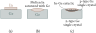
\includegraphics[scale=1]{figures/ch_08/fig_8_11.pdf}
		\caption[]{Fabrication of alloyed p-n junction: (a)---room temperature; (b)---temperature $T\approx\SI{500}{\degreeCelsius}$; (c)---room temperature.}
		\label{fig:8_11}
	\end{center}
	\vspace{-0.8cm}
\end{figure}

The p-n junction can be prepared by diffusing acceptor impurities into an n-type semiconductor or donor impurities into a p-type semiconductor. The diffusion process may be carried out from the
gaseous, liquid, or solid phases. The penetration of the impurity and the depth of the p-n junction is determined by the temperature and the time of the diffusion process. The p-n junction itself is the boundary that separates the regions of different conductivity types.

A widely used method is the epitaxial method of preparing p-n junctions which consists in the deposition via chemical reactions on, for instance, an n-type silicon wafer of a p-type single crystalline silicon film in the gaseous phase or recrystallization from the liquid phase being used for the process.

A method growing in popularity in recent years is the ion implantation method, in which energetic ions of specific impurities (energy in the range of \SIrange{50}{300}{\kilo\electronvolt}) are directed at the semiconductor surface and penetrate into the bulk of it (to a depth of the order of \SIrange{0.1}{0.5}{\micro\metre}, depending on the energy and the type of impurity).

\textbf{Equilibrium state of a p-n junction.} Let the plane MM be the internal boundary between two semiconductor regions of different conductivity type [\fig{8_12}(a)]: to the left is the p-type semiconductor, for instance, p-germanium, with an acceptor concentration $\ab{N}{a}$, and to the right an n-type semiconductor (n-germanium) with a donor concentration $\ab{N}{d}$. For the sake of simplicity we shall assume $\ab{N}{a}=\ab{N}{d}$ to be equal to \SI{e22}{\per\metre\cubed}. Figure \ref{fig:8_12}(b) depicts the change in the acceptor and donor concentrations along the x axis perpendicular to the plane MM. At point $0$ lying in this plane, the acceptor concentration abruptly vanishes and the donor concentration increases abruptly from zero to $\ab{N}{d}$.

\begin{figure}[t]
	\begin{center}
		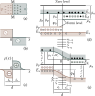
\includegraphics[scale=1.1]{figures/ch_08/fig_8_12.pdf}
		\caption[]{Equilibrium state of p-n junction: (a)---internal boundary MM between p- and n-regions; (b)---impurity distribution in p- and n-regions; (c)---distribution of immobile charges in p-n junction; (d)---position of Fermi levels at the time of imaginary contact of p- and n-regions; (e)---deflection of energy bands in the course of p-n junction formation and formation of a space charge layer.}
		\label{fig:8_12}
	\end{center}
	\vspace{-0.8cm}
\end{figure}

The majority carriers in the n-type region are electrons, and in the p-type region holes. The majority carriers are due almost entirely to ionized donor and acceptor impurity atoms. At temperatures
outside the extreme low temperature range, practically all of those impurity atoms are ionized and, because of that, the electron concentration in the n-region ($\ab{n}{n$0$}$) can be assumed to be equal to the donor concentration $\ab{N}{d}$ ($\ab{n}{n$0$}\approx\ab{N}{d}$), and the hole concentration in the p-region ($\ab{p}{p$0$}$) can be assumed to be equal to the concentration
of the acceptor atoms ($\ab{p}{p$0$}\approx\ab{N}{a}$).

Besides majority carriers those regions contain also minority carriers: the n-region contains holes ($\ab{p}{n$0$}$) and the p-region electrons ($\ab{n}{p$0$}$). Their concentrations may be found from the law of mass action \eqref{eq:5_44}
\begin{equation*}
	\ab{n}{n$0$} \ab{p}{n$0$} = \ab{p}{p$0$} \ab{n}{p$0$} = \ab{n}{i}^2
\end{equation*}

\noindent
where $\ab{n}{i}$ is the concentration of carriers of one sign in the intrinsic semiconductor (germanium). At $\ab{n}{n$0$}=\ab{p}{p$0$}=\SI{e22}{\per\metre\cubed}$ and $\ab{n}{i}=\SI{e19}{\per\metre\cubed}$ we get $\ab{p}{n$0$}=\ab{n}{p$0$}=\SI{e16}{\per\metre\cubed}$.

We see that the hole concentration in the p-region is six orders of magnitude higher than in the n-region. Such a difference in the concentrations of carriers of one type is the cause of diffusion fluxes of electrons from the n-region to the p-region ($\ab{n}{n$\to$p}$) and of holes from the p-region to the re-region ($\ab{p}{p$\to$n}$). The diffusion flux of the electrons out of the n-region imparts a positive charge to this region, and the hole flux from the p-region imparts a negative charge to the p-region. Such charges raise the position of all the energy levels including the Fermi level in the p-region and sink it in the n-region. The electrons continue to flow from the right to the left and the holes from the left to the right until the gradually rising Fermi level of the p-region ($\ab{\mu}{p}$) reaches the level of the gradually sinking Fermi level of the n-region ($\ab{\mu}{n}$).
As soon as those levels are equalized a state of equilibrium is established between the n- and p-regions when the electron flux from the n- to the p-region ($\ab{n}{n$\to$p}$) is compensated by the electron flux from the p- to the n-region ($\ab{n}{p$\to$n}$) and the hole flux from the p- to the n-region ($\ab{p}{p$\to$n}$) is compensated by the hole flux from the n- to the p-region ($\ab{p}{n$\to$p}$):
\begin{equation}\label{eq:8_17}
	\ab{n}{n$\to$p} = \ab{n}{p$\to$n},\quad \ab{p}{p$\to$n} = \ab{p}{n$\to$p}.
\end{equation}

As the electrons leave the contact layer of the n-region, a static positive space charge of ionized donor atoms is left in it [\fig{8_12}(c)]. Denote the width of this layer by $\ab{d}{n}$. As the holes leave the contact layer of the p-region, a static negative space charge of the ionized acceptor atoms is left there. Denote the width of this layer by $\ab{d}{p}$. A contact potential difference $\ab{V}{c}$ is built up across those layers, which constitutes a potential barrier $\varphi_0$ localized in the p-n junction; $\varphi_0$ prevents the electrons from going over from the n- to the p-region and the holes from the p- to the re-region. Calculations show that
\begin{equation}\label{eq:8_18}
	\varphi_0 = \ab{k}{B} T \ln\parenthesis{\frac{\ab{n}{n$0$}}{\ab{n}{p$0$}}} = \ln\parenthesis{\frac{\ab{p}{p$0$}}{\ab{p}{n$0$}}}.
\end{equation}

It follows from \eqn{8_18} that $\varphi_0$ is the greater the greater the ratio of the majority carrier concentration in one region of the p-n junction to the concentration of the carriers of the same type in another region where they are minority carriers. At $\ab{n}{n$0$}=\SI{e22}{\per\metre\cubed}$, $\ab{n}{p$0$}=\SI{e16}{\per\metre\cubed}$, and $T=\SI{300}{\kelvin}$ we see that $\varphi_0\approx\SI{0.45}{\electronvolt}$.

Figure \fig{8_12}(d) shows the energy band pattern of the p- and n-regions at the instant of their imaginary contact, that is, before equilibrium between them has been established. It may be seen from \fig{8_12}(d) that $\ab{\mu}{n}$ lies above $\ab{\mu}{p}$.

Figure \ref{fig:8_12}(e) shows the energy band pattern of those regions after equilibrium has been established. The Fermi levels $\ab{\mu}{n}$ and $\ab{\mu}{p}$ coincide and there is a space charge layer between the p- and n-regions that spreads into the n-region to a depth $\ab{d}{n}$ and into the p-region to a depth $\ab{d}{p}$ forming a potential barrier with the height $\varphi_0=q\ab{V}{c}$. Comparing Figures \ref{fig:8_12}(d) and (e), one may easily see that
\begin{equation}\label{eq:8_19}
	\varphi_0 = \ab{\mu}{n} - \ab{\mu}{p}.
\end{equation}

\noindent
The width of the space charge layer $d=\ab{d}{n}+\ab{d}{p}$, as in the case of the metal-semiconductor contact, is determined by the height
of the potential barrier $\varphi_0$ and by the concentrations of majority carriers in both regions of the p-n junction $\ab{n}{n$0$}$ and $\ab{p}{p$0$}$:
\begin{equation}\label{eq:8_20}
	d = \bracket{\parenthesis{\frac{2\varepsilon\varepsilon_0\varphi_0}{q^2}} \parenthesis{\frac{\ab{n}{n$0$} + \ab{p}{p$0$}}{\ab{n}{n$0$}\ab{p}{p$0$}}}}^{1/2} = \bracket{\parenthesis{\frac{2\varepsilon\varepsilon_0\ab{V}{c}}{q^2}} \parenthesis{\frac{\ab{n}{n$0$} + \ab{p}{p$0$}}{\ab{n}{n$0$}\ab{p}{p$0$}}}}^{1/2}.
\end{equation}

It may, however, be demonstrated that in the p-n junction the barrier width $d$ depends eventually only on the majority carrier concentrations $\ab{n}{n$0$}$ and $\ab{p}{p$0$}$. Indeed, substituting \eqn{5_38} into \eqref{eq:8_18} and the result into \eqn{8_20}, we obtain
\begin{equation*}
	d = \bracket{\parenthesis{\frac{2\varepsilon\varepsilon_0}{q^2}} \parenthesis{\frac{\ab{n}{n$0$} + \ab{p}{p$0$}}{\ab{n}{n$0$}\ab{p}{p$0$}}} \ab{k}{B}T \ln\parenthesis{\frac{\ab{n}{n$0$}\ab{p}{p$0$}}{\ab{n}{i}^2}}}^{1/2}.
\end{equation*}

\noindent
It follows from \eqn{8_20} that the space charge layer width is the greater the less the majority carrier concentration in the n- and p-regions of the semiconductor.

If one of the regions, for instance the n-region, is substantially less doped than the p-region, so that $\ab{n}{n$0$}\ll\ab{p}{p$0$}$, we will obtain from \eqn{8_20} the following:
\begin{equation}\label{eq:8_21}
	d \approx \ab{d}{n} \approx \parenthesis{\frac{2 \varepsilon \varepsilon_0 \varphi_0}{q^2 \ab{n}{n$0$}}}^{1/2}.
\end{equation}

In this case, almost the entire space charge is concentrated in the low-doped (high resistivity) n-region, the same as in the case of a metal-semiconductor contact.

\textbf{Rectifying properties of p-n junctions.} A remarkable property of the p-n junction, on which the operation of most semiconductor devices is based, is its ability to rectify alternating current. Let us discuss this property in more detail.

\textbf{Currents flowing through p-n junction in equilibrium.} In the state of equilibrium, fluxes of majority and minority carriers flow through the p-n junction [\fig{8_12}(c)]. These fluxes are such that the flux of electrons---majority carriers---flowing from the n- to the p-region ($\ab{n}{n$\to p$}$) is, according to \eqn{8_18}, equal to the flux of electrons---minority carriers---flowing from the p- to the n-region ($\ab{n}{p$\to n$}$). In the same way, the flux of holes---majority carriers---flowing from the p- to the n-region ($\ab{p}{p$\to n$}$) is equal to the flux of holes---minority carriers---flowing from the n- to the p-region ($\ab{p}{n$\to p$}$).
Denote the current densities corresponding to those fluxes as follows: the flux $\ab{n}{n$\to p$}$ corresponds to $\ab{i}{n}$, $\ab{n}{p$\to n$}$ to $\ab{i}{p}$ and $\ab{p}{n$\to p$}$ to $\ab{i}{p-eq}$. In accordance with \eqn{8_17} we can write
\begin{equation}\label{eq:8_22}
	\ab{i}{n} = \ab{i}{n-eq},\quad \ab{i}{p} = \ab{i}{p-eq}.
\end{equation}

\noindent
Adding the right- and left-hand sides of those equations, we obtain
\begin{equation*}
	\ab{i}{n} + \ab{i}{p} = \ab{i}{n-eq} + \ab{i}{p-eq}.
\end{equation*}

\noindent
The left-hand side of the relation expresses the component of the full current due to the majority carriers, and the right hand side the component due to the minority carriers. The full current flowing through the p-n junction will evidently be zero:
\begin{equation}\label{eq:8_23}
	i = (\ab{i}{n} + \ab{i}{p}) - (\ab{i}{n-eq} + \ab{i}{p-eq}) = 0.
\end{equation}

\begin{figure}[t]
	\begin{center}
		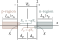
\includegraphics[scale=1.0]{figures/ch_08/fig_8_13.pdf}
		\caption[]{Calculating minority carrier currents flowing through equilibrium p-n junction.}
		\label{fig:8_13}
	\end{center}
	\vspace{-0.8cm}
\end{figure}

Let us calculate $\ab{i}{n-eq}$ and $\ab{i}{p-eq}$. To this end, cut out a unit area $S$ of the left boundary $1$ of the p-n junction (\fig{8_13}). Using
it as a base, build a cylinder with the side $\ab{L}{n}/\ab{\tau}{n}$, where $\ab{L}{n}$ is the diffusion length of the electrons in the p-region and $\ab{\tau}{n}$ their average lifetime. Since the diffusion length is the average distance the carrier
passes during its lifetime, the ratio $\ab{L}{n}/\ab{\tau}{n}$, evidently, expresses the average speed of electrons diffusing from the bulk of the p-region, where their concentration is $\ab{n}{p$0$}$ to the boundary $1$, where they are drawn into the contact field and transported to the n-region.

The number of electrons contained in the cylinder is equal to its volume $\ab{L}{n}/\ab{\tau}{n}$ multiplied by the electron concentration $\ab{n}{p$0$}$, that is $\ab{L}{n}\ab{n}{p$0$}/\ab{\tau}{n}$. All those electrons will pass through the unit area $S$ in one second and will be transported to the n-region establishing a current with a density
\begin{equation}\label{eq:8_24}
	\ab{i}{n-eq} = \frac{q \ab{L}{n} \ab{n}{p$0$}}{\ab{\tau}{n}}.
\end{equation}

One may similarly calculate $\ab{i}{n-eq}$ by building a cylinder of unit base with the side equal to $\ab{L}{n}/\ab{\tau}{n}$ at the boundary $2$ of the p-n junction:
\begin{equation}\label{eq:8_25}
	\ab{i}{p-eq} = \frac{q \ab{L}{p} \ab{p}{n$0$}}{\ab{\tau}{p}}.
\end{equation}

Hence, in the state of equilibrium in the p-n junction,
\begin{equation}\label{eq:8_26}
	\begin{split}
		\ab{i}{n} &= \ab{i}{n-eq} = \frac{q \ab{L}{n} \ab{n}{p$0$}}{\ab{\tau}{n}}\\
		\ab{i}{p} &= \ab{i}{p-eq} = \frac{q \ab{L}{p} \ab{p}{n$0$}}{\ab{\tau}{p}}.
	\end{split}
\end{equation}

\textbf{Forward current.} Apply a forward voltage $V$ to a p-n junction in a state of equilibrium [\fig{8_14}(a)], by connecting the positive terminal of the power supply to the p-region and the negative terminal to the n-region [\fig{8_14}(b)]. This voltage brings the potential barrier for the majority carriers down to $\varphi0-qV$. Therefore, the electron flux from the n- to the p-region ($\ab{n}{n$\to$p}$), and the hole flux from the p- to the n-region will increase $e^{qV/(\ab{k}{B}T)}$ times with the resulting similar increase in the majority carriers current densities $\ab{i}{n}$ and $\ab{i}{p}$:
\begin{equation*}
	\ab{i}{n} = \frac{q\ab{L}{n} \ab{n}{p$0$}}{\ab{\tau}{n}}\, e^{qV/(\ab{k}{B}T)},\quad \ab{i}{p} = \frac{q\ab{L}{p} \ab{p}{n$0$}}{\ab{\tau}{p}}\, e^{qV/(\ab{k}{B}T)}.
\end{equation*}

\begin{figure}[t]
	\begin{center}
		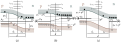
\includegraphics[scale=1.0]{figures/ch_08/fig_8_14.pdf}
		\caption[]{Rectifying action of p-n junction: (a)---equilibrium state of p-n junction; (b)---forward voltage applied to p-n junction; (c)---reverse voltage applied to p-n junction.}
		\label{fig:8_14}
	\end{center}
	\vspace{-0.8cm}
\end{figure}

At the same time the current densities of minority carriers $\ab{i}{n-eq}$ and $\ab{i}{p-eq}$ whose magnitude is independent of the p-n junction's barrier height shall remain the same as expressed by formulae \eqref{eq:8_26}. Therefore, the total current flowing through the p-n junction, to which a forward voltage $V$ has been applied and termed \textit{forward current} $\ab{i}{f}$, will now be not zero but
\begin{equation}\label{eq:8_27}
	\ab{i}{f} = (\ab{i}{n} + \ab{i}{p}) - (\ab{i}{n-eq} + \ab{i}{p-eq}) = q \parenthesis{ \frac{\ab{L}{n} \ab{n}{p$0$}}{\ab{\tau}{n}} + \frac{\ab{L}{p} \ab{p}{n$0$}}{\ab{\tau}{p}} } \bracket{e^{qV/(\ab{k}{B}T)} - 1}.
\end{equation}

\textbf{Reverse current.} Apply now a reverse voltage $-V$ to the p-n junction, by connecting the negative terminal of the power supply to the p-region and the positive one to the n-region [\fig{8_14}(c)]. This voltage raises the potential barrier of the p-n junction to $\varphi_0+qV$, with the result that the fluxes of the majority carriers $\ab{n}{n$\to$p}$  and $\ab{p}{p$\to$n}$ decrease $e^{qV/(\ab{k}{B}T)}$ times together with their currents $\ab{i}{n}$ and $\ab{i}{p}$. The latter will be equal to:
\begin{equation*}
	\ab{i}{n} = \frac{q \ab{L}{n} \ab{n}{p$0$}}{\ab{\tau}{n}}\, e^{-qV/(\ab{k}{B}T)},\quad \ab{i}{p} = \ab{i}{p-eq} = \frac{q \ab{L}{p} \ab{p}{n$0$}}{\ab{\tau}{p}}\, e^{-qV/(\ab{k}{B}T)}.
\end{equation*}

The total current flowing in the p-n junction termed \textit{reverse current} $\ab{i}{r}$ will be
\begin{equation}\label{eq:8_28}
	\ab{i}{r} = (\ab{i}{n} + \ab{i}{p}) - (\ab{i}{n-eq} + \ab{i}{p-eq}) = q \parenthesis{ \frac{\ab{L}{n} \ab{n}{p$0$}}{\ab{\tau}{n}} + \frac{\ab{L}{p} \ab{p}{n$0$}}{\ab{\tau}{p}} } \bracket{e^{-qV/(\ab{k}{B}T)} - 1}.
\end{equation}

\textbf{Current-voltage characteristic (CVC).} Combining \eqns{8_27}{8_28}, we obtain the equation for the current-voltage characteristic of the p-n junction:
\begin{equation}\label{eq:8_29}
	i = q \parenthesis{ \frac{\ab{L}{n} \ab{n}{p$0$}}{\ab{\tau}{n}} + \frac{\ab{L}{p} \ab{p}{n$0$}}{\ab{\tau}{p}} } \bracket{\pm e^{-qV/(\ab{k}{B}T)} - 1},
\end{equation}

\noindent
where $V>0$ is the forward voltage, and $V<0$ the reverse voltage.

Let us analyse this formula. With the increase in the reverse voltage $-V$, the exponent $e^{-qV/(\ab{k}{B}T)}\to 0$ and the expression $\bracket{e^{-qV/(\ab{k}{B}T)} - 1}\to -1$. Accordingly, the current density $\ab{i}{r}$ tends to its limit
\begin{equation}\label{eq:8_30}
	\ab{i}{eq} = - q \parenthesis{ \frac{\ab{L}{n} \ab{n}{p$0$}}{\ab{\tau}{n}} + \frac{\ab{L}{p} \ab{p}{n$0$}}{\ab{\tau}{p}} },
\end{equation}

\noindent
termed \textit{saturation current density}. Practically, this value is reached already at $qV\approx 4\ab{k}{B}T$, that is for $V\approx\SI{0.1}{\volt}$. It follows from \eqn{8_30}, that $\ab{i}{eq}$ is determined by the minority carrier fluxes through the p-n junction. Since their concentrations are not large, $\ab{i}{eq}$ is a small quantity.
For germanium p-n junctions of the type discussed here ($\ab{n}{n$0$}\approx\ab{p}{p$0$}\approx\SI{e22}{\per\metre\cubed}$) at room temperature, $\ab{i}{eq}$ it is of the order of \SI{e-2}{\ampere\per\metre\squared}; for silicon p-n junctions it is much less.

When a forward voltage $V$ is applied to the p-n junction, the current density through it increases exponentially and reaches big values already at small voltages. Substituting \eqn{8_30} into \eqref{eq:8_29}, we obtain:
\begin{equation}\label{eq:8_31}
	i = \ab{i}{eq} \bracket{\pm e^{-qV/(\ab{k}{B}T)} - 1}.
\end{equation}

Figure \ref{fig:8_15} shows the plot of a current-voltage characteristic of a p-n junction which corresponds to equations \eqns{8_29}{8_31}.

\begin{figure}[t]
	\begin{center}
		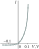
\includegraphics[scale=1.0]{figures/ch_08/fig_8_15.pdf}
		\caption[]{Current-voltage characteristic of p-n junction.}
		\label{fig:8_15}
	\end{center}
	\vspace{-0.8cm}
\end{figure}

It is drawn to different scales for the forward and reverse branches since should the same scale be used for the reverse current as for the forward current the reverse branch would coincide with the $x$ axis. Indeed, for $\ab{V}{r}=-\SI{0.5}{V}$, the reverse current density is $\ab{i}{r}\approx\ab{i}{eq}$, and for $\ab{V}{f}=\SI{0.5}{V}$, the forward current density it $\ab{i}{f}\approx\ab{i}{eq}\,e^{20}\approx\ab{i}{eq}\num{e9}$, since at $T=\SI{300}{\kelvin}$ (room temperature) $\ab{k}{B}T\approx\SI{0.025}{\electronvolt}$.
As we see, the rectification coefficient at such a voltage is $\ab{i}{f}/\ab{i}{r}\approx\num{e9}$ and this proves that a p-n junction exhibits a practically unidirectional conductivity.

\textbf{Deterioration of rectifying properties at high temperatures.} According to \eqn{5_44}
\begin{equation*}
	\ab{p}{n$0$} = \frac{\ab{n}{i}^2}{\ab{n}{n$0$}},\quad \ab{n}{p$0$} = \frac{\ab{n}{i}^2}{\ab{p}{p$0$}}
\end{equation*}

\noindent
where
\begin{equation*}
	\ab{n}{i} = 2 \parenthesis{ \frac{2\pi\sqrt{\ab{m}{n}\ab{m}{p}} \ab{k}{B}T}{h^2} }^{1/2}\, e^{-\ab{E}{g}/(\ab{k}{B}T)}.
\end{equation*}

\noindent
It may easily be seen that $\ab{n}{i}$ will rise rapidly with the increase in temperature while $\ab{n}{n$0$}\approx\ab{N}{d}$ and $\ab{p}{p$0$}\approx\ab{N}{a}$ will remain practically constant. Therefore, at some temperature $\ab{n}{i}$ may become as high as $\ab{n}{n$0$}$ or $\ab{p}{p$0$}$.
Then, the concentrations of the minority carriers will be as high as the concentrations of the majority carriers: $\ab{p}{n$0$}=\ab{n}{i}^2/\ab{n}{n$0$}\approx=\ab{n}{n$0$}^2/\ab{n}{n$0$}=\ab{n}{n$0$}$ and $\ab{n}{p$0$}=\ab{n}{i}^2/\ab{p}{p$0$}\approx\ab{p}{p$0$}^2/\ab{p}{p$0$}=\ab{p}{p$0$}$.
The potential barrier in the p-n junction which is responsible for its rectifying properties will then cease to exist:
\begin{equation*}
	\varphi_0 = \ab{k}{B}T \ln\parenthesis{ \frac{\ab{n}{n$0$}}{\ab{p}{p$0$}} } \approx \ab{k}{B}T \ln(1) \approx 0,
\end{equation*}

\noindent
together with the ability of the junction to rectify alternating current. It follows from \eqn{5_37}, that the corresponding temperature will be the higher the higher the forbidden band width $\ab{E}{g}$ of the semiconductor. For germanium p-n junctions ($\ab{E}{g}=\SI{0.62}{\electronvolt}$), the highest operational temperature is $75$-\SI{90}{\degreeCelsius}; for silicon p-n junctions ($\ab{E}{g}=\SI{1.12}{\electronvolt}$) it can be as high as \SI{150}{\degreeCelsius}.

\textbf{Breakdown in p-n junctions.} If the reverse voltage is continuously increased, a voltage $\ab{V}{b.d}$ will be reached, at which the resistance of the barrier layer drops drastically and the reverse current jumps up. This phenomenon became known as the p-n junction breakdown (\fig{8_16}).

\begin{figure}[t]
	\begin{center}
		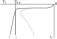
\includegraphics[scale=1.0]{figures/ch_08/fig_8_16.pdf}
		\caption[]{p-n junction breakdown: $1$---thermal, $2$---avalanche; $3$---tunnel.}
		\label{fig:8_16}
	\end{center}
	\vspace{-0.8cm}
\end{figure}

There are different types of breakdown: thermal, tunnel (or Zener), and the avalanche breakdown in accordance with the nature of the physical processes that cause the reverse current to grow abruptly.

\textit{Thermal breakdown} occurs when the heat generated by the reverse current flowing through the p-n junction is not completely removed from it and raises its temperature. A rising temperature leads to an increase in the reverse current and this, in its turn, raises the temperature still further, etc. This progressive process results eventually in thermal breakdown. The character of the increase in current during such a breakdown is depicted in \fig{8_16}, curve $1$.

When the electric field intensity in the p-n junction is high enough, impact ionization of the atoms of the semiconductor may take place. This will result in an avalanche-type increase in the carrier concentration and in the \textit{avalanche breakdown}; the character of the increase in current is shown in \fig{8_16}, curve $2$.

In a narrow p-n junction already at comparatively low reverse voltages, an electric field may be established high enough for the tunnelling of the electrons through the p-n barrier to take place. The resulting breakdown is termed \textit{tunnel}, or \textit{Zener}, \textit{breakdown} and the character of current increase $\ab{i}{r}(V)$ for this case is shown in \fig{8_16}, curve $3$.

In most cases, the p-n junction breakdown is a harmful effect that limits the practical use of the junction. At the same time, the effect was utilized to develop a wide range of semiconductor devices known as Zener diode voltage regulators, which will be discussed in the following section.

\section{Physical principles of semiconductor p-n junction devices}\label{sec:77}

As had already been stated before, the rapid progress in semiconductor electronics was the direct result of the development of the p-n junction technology on which the design of various semiconductor devices is based. Let us discuss the general principles of such devices.

\textbf{Rectifier diodes.} The nonlinear current-voltage characteristic of the p-n junction (\fig{8_15}) enables it to be used to rectify alternating current. A two-terminal semiconductor device fulfilling such function is termed \textit{semiconductor rectifier diode}. Figure \ref{fig:8_17} shows the principal schematic diagram of such a diode. It consists of a p-n junction $1$, passive n- and p-regions $2$ and $3$, and ohmic contacts $4$. The high-resistivity region of the crystal is termed \textit{base} of the diode. In our case it is the n-region $3$ of the width $W$.

\begin{figure}[t]
	\begin{center}
		\includegraphics[scale=1.0]{figures/ch_08/fig_8_17.pdf}
		\caption[]{Schematic representation of a rectifier diode: $1$---p-n junction, $2$ and $3$---passive regions, $4$---ohmic contacts.}
		\label{fig:8_17}
	\end{center}
	\vspace{-0.8cm}
\end{figure}

Nowadays, p-n junction rectifier diodes are made almost exclusively of silicon. The efficiency of such diodes is almost $100$ percent and in combination with their low weight, small dimensions, ease of servicing, etc. this made them a very widely used device for such applications. Various diode types are designed to rectify currents from several milliamperes to several hundred or thousand amperes.
For greater currents the diodes are connected in parallel. The maximum reverse voltage for various types lies in the range from \SIrange{50}{600}{\volt}. It may be much higher for special diode types. For use in high-voltage rectifiers the diodes are assembled in-series in stacks. The reverse currents of various rectifier types lie in the range from fractions of a microampere to tens of milliamperes.

\textbf{Impulse and high-frequency diodes.} The second very important field of application of the semiconductor diodes is the field of impulse electronics, computer electronics, automation, VHF electronics, etc. In such applications, the diode is required to process pulses of minimum duration and of maximum repetition rate. Therefore, one of the main requirements of diodes designed for such circuits is the speed of operation, that is, switching speed from the direct to the reverse state. To find what lies at the origin of this speed let us discuss the physical processes that take place when a p-n junction is switched.

\begin{figure}[t]
	\begin{center}
		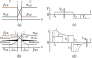
\includegraphics[scale=1.0]{figures/ch_08/fig_8_18.pdf}
		\caption[]{Transient processes in diode: (a)---majority and minority carrier distributions; (b)---minority carrier injection by forward voltage and their diffusion into the bulk of semiconductor; (c, d)---variations of forward and reverse voltages and currents in a diode switched on in the forward direction and reswitched to reverse direction.}
		\label{fig:8_18}
	\end{center}
	\vspace{-0.8cm}
\end{figure}

Figure \ref{fig:8_18}(a) shows the distribution of the majority and minority carriers in the p- and n-regions of an equilibrium p-n junction. When a direct voltage $V$ is applied to the diode, the potential barrier of its p-n junction sinks by $qV$ and the majority carrier flux through the junction increases $e^{qv/\ab{k}{B}T}$ times, with the result that the hole concentration at boundary $1$ and the electron concentration at boundary $2$ rise to the values of $\ab{p}{n}(0)\gg\ab{p}{n$0$}$ and $\ab{n}{p}(0)\gg\ab{n}{p$0$}$, respectively [\fig{8_18}(b)].
For the direct current to flow, it is necessary for those carriers to be drawn into the bulk of the semiconductor: the holes should be drawn into the n-region and the electrons into the p-region. The recombination of those minority carriers takes place inside the regions, or on the contacts if the width of the regions is small in comparison with their diffusion length. The removal of the minority carriers proceeds either by means of diffusion, whose rate is the higher the greater the concentration gradient of holes ($\diffin{p}{x}$) at boundary $2$ and that of electrons ($\diffin{n}{x}$) at boundary $1$ or in special diode types by means of drift in built-in electric fields. At the initial moment after the forward voltage had been applied
[\fig{8_18}(c)], this gradient is extremely high, since the holes transported to the n-region and the electrons transported to the p-region are concentrated in narrow layers close to boundaries $2$ and $1$. Therefore, the initial forward current in the diode is high, being limited practically only by the resistance of its passive regions [plateau $1$
in \fig{8_18}(d)]. As the holes enter the n-region and the electrons the p-region, their concentration gradient drops and so does the forward current [\fig{8_18}(e)]. After a time equal to the minority
carrier lifetime $\tau$ (or to the transit time of the minority carriers from the boundaries $1$ and $2$ to the contacts $4$, which is even shorter), a steady-state (independent in time) distribution of the holes in the n-region and of the electrons in the p-region is established [\fig{8_18}(b)] and the forward current assumes its normal value [\fig{8_18}(d)].

When the diode is switched from the forward to the reverse state [\fig{8_18}(c)], the initial reverse current is very high since the minority carrier concentrations at boundaries $2$ and $1$, which are
responsible for this current, are high: the magnitude of the current is actually limited by the resistance of the passive regions of the diode [plateau $2$ in \fig{8_18}(d)]. In the course of time, the excess carriers at the boundaries gradually dissolve, their concentrations drop to equilibrium values ($\ab{p}{n$0$}$ and $\ab{n}{p$0$}$), and the reverse current assumes its normal value [\fig{8_18}(d)]. This process lasts about the same time as the first (lifetime or transit time).

Thus, when the diode is switched, transient processes (of carrier accumulation in the forward biased diode and of carrier dissipation in the reverse biased diode) take place in it, limiting its switching speed. Since the duration of those processes is approximately equal to the minority carrier lifetime $\tau$, and since a reduction in $\tau$ increases the switching speed, the tendency is to make $\tau$ as short as possible. Another method is to reduce the transit time of carriers by making the diodes as thin as possible (several microns or less).

On the basis of the aforesaid, we can draw the conclusion that, a p-n junction behaves with respect to a short alternating signal as a resistance $R$ located in the barrier layer shunted by the capacitance $C$ of the p-n junction (\fig{8_19}). When a forward bias is applied, the initial current through the diode is mainly the current which charges the capacitor $C$. This current can be quite high. When the diode is switched to the reverse bias, the initial reverse current is mainly the discharge current of the capacitor $C$ and it too can be quite high. To improve the speed of the diode and its high-frequency performance it is evidently necessary to reduce the p-n junction capacitance $C$. This is done by reducing the area of the p-n junction to the minimum. This measure together with other measures enabled the switching speeds of modern diodes to be reduced to approximately \SI{e-9}{\second} and the operating frequencies to be raised to \SI{e9}{\hertz}.

\begin{figure}[!t]
	\begin{minipage}[t]{0.48\linewidth}
		\begin{center}
            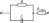
\includegraphics[scale=0.98]{figures/ch_08/fig_8_19.pdf}
            \caption[]{Equivalent circuit of diode: $R$---non-linear resistance of p-n junction, $C$---capacitance of p-n junction; $\ab{R}{ohm}$---ohmic resistance of passive regions and contacts.}
            \label{fig:8_19}
		\end{center}
	\end{minipage}
	\hfill{ }%\hspace{-0.1cm}
	\begin{minipage}[t]{0.48\linewidth}
		\begin{center}
			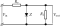
\includegraphics[scale=0.98]{figures/ch_08/fig_8_20.pdf}
			\caption[]{Circuit diagram of the simplest voltage regulator using a silicon Zener diode $Z$.}
			\label{fig:8_20}
		\end{center}
	\end{minipage}
\vspace{-0.3cm}
\end{figure}

\textbf{Voltage regulators.} A small increase in the reverse voltage in the prebreakdown range causes a substantial increase in the reverse current (see \fig{8_16}). This effect is being used to stabilize voltage and the device is called the \textit{Zener diode regulator}.

Figure \ref{fig:8_20} depicts the simplest circuit diagram of a dc voltage stabilizer utilizing a Zener diode. When the input voltage $\ab{F}{in}$ is increased, the diode's resistance drops drastically, and the current in the circuit of the voltage drop resistor $\ab{R}{v}$ increases, causing the voltage drop across it to increase; the voltage across the load resistance $\ab{R}{l}$ (the output voltage $\ab{V}{out}$) may remain practically constant. Power supplies using Zener diodes are now quite a match for normal cells.

\textbf{Tunnel diodes.} There is another very interesting and practically important type of semiconductor devices, the so-called \textit{tunnel diode}, which utilizes the quantum mechanical effect of electrons tunnelling through a narrow potential barrier. The diodes are constructed from heavily doped degenerate semiconductor material in which the Fermi level lies not in the forbidden band, but just like in metals in the conduction band of an n-type semiconductor or in the valence band of a p-type semiconductor. Figure \ref{fig:8_21}(a) shows the energy-band diagram of a tunnel diode in the state of equilibrium. We see that there is a partial overlapping of the valence band of the p-region and the conduction band of the n-region. This makes possible the tunnelling of electrons from the n-region to the p-region (flux $1$) and from the p-region to the n-region (flux $2$). Flux $1$ constitutes the reverse tunnelling current and flux $2$ the direct current. In the absence of an external field, those currents are equal and the total current through the junction is zero.

\begin{figure}[t]
	\begin{center}
		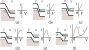
\includegraphics[scale=1.1]{figures/ch_08/fig_8_21.pdf}
		\caption[]{Principle of operation and current-voltage characteristic of the tunnel diode.}
		\label{fig:8_21}
	\end{center}
	\vspace{-0.8cm}
\end{figure}

When a direct voltage is applied to the junction, the overlapping of the bands becomes smaller [\fig{8_21}(b)] and, because of this, flux $2$ exceeds flux $1$ and a direct current passes through the junction increasing with the direct voltage $V$ until a maximum is reached, corresponding to a voltage at which the bottom of the conduction band of the n-region coincides with the Fermi level of the p-region [\fig{8_21}(c)]. When $V$ is increased still further, the direct current diminishes because of the decrease in the number of occupied states of the n-region lying opposite the free states of the p-region [\fig{8_21}(d)]. When at a voltage $V$, the bottom of the conduction band of the n-region, coincides with the top of the valence band of the p-region, the overlapping of the bands ceases [\fig{8_21}(e)] and the tunnel current turns zero, but a small direct current appears as in a usual diode. It rises rapidly with a further increase in $V$ in accordance with \eqn{8_27} [\fig{8_21}(f)].

A remarkable property of the tunnel diodes is the negative differential resistance region $1$-$2$ on the current-voltage characteristic similar to that of the Gunn diode. This makes it possible to use those diodes for the generation of VHF oscillations up to frequencies of about \SI{e11}{\hertz}. The tunnel diode was one of the first devices with a switching time of a fraction of a nanosecond (\SI{e-10}{\second}) and this enabled it to be used in impulse circuits of digital computers and in various automation circuits. Only the majority carriers work in the tunnel diodes and this makes them much less sensitive to ionizing radiation than the bipolar semiconductor devices, this fact being of special importance for space explorations.

The development of the tunnel diodes is an excellent illustration of the fact that the quantum mechanics, formerly an exotic science, became for the modern engineer a powerful tool, mastered in order to be able to take an active part in the progress of modern technology.

\textbf{Transistors.} Rapid progress in semiconductor electronics became possible only after the invention in 1948-1949 by J. Bardeen, W. H. Brattain, and W. Shockley of the semiconductor amplifier---the transistor---whose characteristics and whose designation were similar to those of the vacuum tube but which had some substantial advantages over the latter.

Figure \ref{fig:8_22}(a) shows the schematic representation of an n-p-n junction transistor. The transistor is made of three regions: the left n-region E termed \textit{emitter}, the middle p-region B termed \textit{base}, and the right n-region C termed \textit{collector}. Those regions are separated by two p-n junctions: the emitter and collector junctions. By means of ohmic contacts the transistor is connected into the circuit: one of the possible connections (the common base connection) is shown in \fig{8_22}(a), where $\ab{R}{in}$ is the equivalent input resistance of the transistor and $\ab{R}{out}$ its equivalent output resistance. It may be seen that the emitter p-n junction, is biased in the forward and the collector in the reverse direction.

\begin{figure}[t]
	\begin{center}
		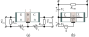
\includegraphics[scale=1.2]{figures/ch_08/fig_8_22.pdf}
		\caption[]{Schematic representation of n-p-n junction transistor and its connection into circuit.}
		\label{fig:8_22}
	\end{center}
	\vspace{-0.8cm}
\end{figure}

To understand the physical principles of transistor operation let us turn again to \fig{8_18}(b). When a forward bias is applied to the emitter p-n junction, the concentrations of the majority carriers---of electrons in the p-region and of holes in the n-region---increase drastically as compared with their equilibrium concentrations. This phenomenon is termed \textit{minority carrier injection} and serves
as the basis for transistor operation.

The electrons injected from the emitter E into the base B [\fig{8_22}(a)] diffuse to the collector C; with a base that is narrow in comparison with the minority carrier diffusion length, practically all the injected electrons will reach the collector junction and will be drawn in by its field into the collector circuit of the transistor. Therefore, the collector current $\ab{I}{c}$ will be approximately equal to the emitter current $\ab{I}{e}$: $\ab{I}{c}=\alpha\ab{I}{e}$, where $\alpha\approx 1$ is the common base current amplification factor.

Now imagine that an external signal $\ab{V}{in}$ small in comparison with the bias voltage $V$ is applied to the input resistance $\ab{R}{in}$. The input current---the emitter signal current---will be $\ab{I}{e}=\ab{V}{in}/\ab{R}{in}$ and the output voltage---the signal voltage across the collector junction (or the equivalent collector resistance $\ab{R}{out}$)---will be $\ab{\widetilde{V}}{out} = \ab{\widetilde{I}}{c}\ab{R}{out}=\alpha\ab{\widetilde{I}}{c}\ab{R}{out}$.
Therefore, the voltage amplification factor $\ab{\alpha}{V}$ of the transistor in the common base connection will be
\begin{equation*}
	\ab{\alpha}{V} = \frac{\ab{\widetilde{V}}{in}}{\ab{\widetilde{V}}{out}} = \alpha \frac{\ab{R}{out}}{\ab{R}{in}} \approx \frac{\ab{R}{out}}{\ab{R}{in}}.
\end{equation*}

Since $\ab{R}{in}$ is a small differential resistance of a forward-biased p-n junction and $\ab{R}{out}$ is an enormous resistance of a reverse-biased junction ($\ab{R}{out}>\ab{R}{in}$), $\ab{\alpha}{V}\gg 1$ and may be as high as \num{e5} (for dc current). Since in this connection only the voltage is amplified, the same will be the power amplification factor $\ab{\alpha}{P}=\ab{P}{out}/\ab{P}{in}\approx\ab{\alpha}{V}$.
The source of the additional signal power dissipated in the collector circuit is the collector power supply $\ab{V}{c}$.

Figure \ref{fig:8_22}(b) shows the transistor connected into a common emitter circuit. In this case the signal from the source S is applied between the emitter and the base, the output signal being taken off the emitter and the collector. The input signal affects the emitter $\ab{\widetilde{I}}{e}$, the collector $\ab{\widetilde{I}}{c}$, and the base $\ab{\widetilde{I}}{b}$ currents, the latter being the difference of the former two ($\ab{\widetilde{I}}{b}=\ab{\widetilde{I}}{e}-\ab{\widetilde{I}}{c}$).
Since $\ab{\widetilde{I}}{c}= \alpha\ab{\widetilde{I}}{e}$, it follows that the \textit{common emitter current amplification factor}
\begin{equation*}
	\beta = \frac{\ab{\widetilde{I}}{c}}{\ab{\widetilde{I}}{b}} = \frac{\ab{\widetilde{I}}{c}}{\ab{\widetilde{I}}{e}\ab{\widetilde{I}}{c}} = \frac{\alpha}{1 - \alpha}
\end{equation*}

\noindent
can be made very high ($\sim\num{e4}$), but from considerations of stability and of frequency response, it is usually held in modern transistors
in the range from $40$ to $100$.

Transistors have found universal application in electronics: in low- and high-frequency amplifier and oscillator circuits, in switching circuits, in triggers and multivibrators, in low- and high-frequency detector circuits, etc. Almost the whole of modern commercial and special-purpose electronics is based on semiconductor devices the most important of which is the transistor.

\textbf{Photoelectric devices. p-n junction photocells.} When a p-n junction is illuminated an emf is established in it. This phenomenon is utilized in barrier layer photocells which may serve as indicators of radiative energy independent of external power sources and as converters of radiative energy into electrical energy.

Figure \ref{fig:8_23}(a) shows the schematic representation of a photocell. A narrow diffused n-layer is fabricated on the surface of a p-type semiconductor wafer so that a p-n junction is formed. In the absence of illumination, the p-n junction is in the state of equilibrium and an equilibrium potential barrier $q\ab{V}{c}$ [\fig{8_23}(b)] is established in it. When the junction is illuminated, electron-hole pairs are generated mostly in the p-region because light passes through the narrow n-layer without absorption. The electrons generated in the p-region diffuse to the p-n junction and are drawn in by the contact field and transported to the n-region. The holes are unable to surmount the barrier $q\ab{V}{c}$ and remain in the p-region. Because of that, the p-region acquires a positive charge and the n-region a negative one, and an additional forward voltage $\ab{V}{ph}$ is established across the junction. The term for it is \textit{photo-emf}, or \textit{photovoltage}.

\begin{figure}[t]
	\begin{center}
		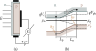
\includegraphics[scale=1.0]{figures/ch_08/fig_8_23.pdf}
		\caption[]{Semiconductor barrier layer photocell: (a)---schematic representation; (b)---energy band pattern of p-n junction.}
		\label{fig:8_23}
	\end{center}
	\vspace{-0.8cm}
\end{figure}

At present the most efficient converters of solar energy are silicon photocells (solar batteries). They are used as power supplies for receivers and transmitters installed on satellites and even on the ground. Calculations show the maximum efficiency (theoretical) of the silicon energy converters to be as high as $22\%$-$23\%$. The efficiency of the best modern types is about $15\%$. Germanium, copper oxide, selenium, silver sulfide, sulfurous thallium and other semiconductor photodiodes are widely used as indicators of radiative energy. Their integral (in the entire spectrum) sensitivity is much higher (\num{e2}-\num{e3} times) than that of the external photoeffect cells. Their main disadvantage is their great inertiality.

\textbf{Photodiodes.} The photodiode is a photocell connected into a circuit in-series with an external power supply [\fig{8_24}(a)]. In the absence of illumination $I$, a negligible so-called \textit{dark current} flows through the junction [\fig{8_24}(b)]. When the p-n junction is illuminated, excess carriers are generated and the current rises in proportion to $I$ causing a voltage drop across the load resistor $\ab{R}{l}$. Substantial advantages of the photodiodes over the external photoeffect elements are smaller dimensions and lower weight, high integral sensitivity and low operating voltage.

\begin{figure}[t]
	\begin{center}
		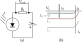
\includegraphics[scale=1.0]{figures/ch_08/fig_8_24.pdf}
		\caption[]{Photodiode: circuit diagram (a) and current-voltage characteristic (b).}
		\label{fig:8_24}
	\end{center}
	\vspace{-0.8cm}
\end{figure}

\textbf{Luminescent diodes.} The passage of a forward current through the p-n junction involves, as we know, minority carrier injection: of electrons into the p-region and of holes into the n-region. The injected carriers recombine with the majority carriers of the respective region, their intensity decreasing with the distance from the p-n junction [\fig{8_18}(b)]. In many semiconductors, the recombination is nonradiative: the energy liberated in the recombination process is absorbed by the crystal lattice, that is, turns eventually into heat. However, in such semiconductors as SiC, GaAs, InAs, GaP, and InSb, the recombination is radiative: the energy of recombination is liberated in the form of radiation quanta, photons.

Because of that a forward current flowing through the p-n junction made of such materials is accompanied by the emission of light from the junction region.

This phenomenon is utilized in the luminescent diodes. Such diodes are used in displays, they may be used in computers for data input and output and  in other applications requiring reliable luminous indicators. Low operating voltages, low power consumption and a long service life are the advantages of the light emission diodes over other electroluminescent light sources.

\textbf{Semiconductor lasers.} In recent years, intensive work has been in progress on the semiconductor sources of coherent radiation---\ie, semiconductor lasers---which open up possibilities for the direct conversion of electric energy into the energy of coherent radiation.

In Figure \ref{fig:8_25}(a), the solid line shows the electron distribution corresponding to the equilibrium state and the dotted line the distribution corresponding to the nonequilibrium state, in which the concentrations of electrons in the conduction band and of the holes in the valence band are above the equilibrium values. Such band occupancy, corresponding to population inversion, is shown in \fig{8_25}(b). The peculiar point about it is that the light quanta with the energy $\hslash\omega=\ab{E}{g}$ ($\ab{E}{g}$ is the forbidden band width) cannot be absorbed by the system. Indeed, such an absorption involves the transfer of an electron from the top level of the valence band to the lowest level of the conduction band. Since there are practically no electrons on the top levels of the valence band and no vacant states at the bottom of the conduction band, the probability of such a process is extremely small. This creates favourable conditions for the stimulated emission and for an avalanche of photons. The light quantum $1$ [\fig{8_25}(b)] stimulates the recombination of the electron and the hole (\ce{\alpha}-transition), which results in the emission of an identical quantum $2$. Since the quanta are not absorbed by the system, they subsequently stimulate the emission of two new quanta, etc. To make one photon take part in many stimulated emission acts, two strictly parallel mirrors $1$ and $2$ [\fig{8_25}(c)] are arranged on the opposite sides of the laser crystal to reflect the incident photons and return them into the crystal. Only those photons are amplified, which move strictly along the $00'$ axis, for only such photons are repeatedly reflected by mirrors $1$ and $2$.
All other photons leave the active laser space immediately or after a limited number of reflections [in \fig{8_25}(c) such photons are shown by dotted lines]. The result is a highly directional and highly monochromatic beam of radiation along the $00'$ axis.

\begin{figure}[t]
	\begin{center}
		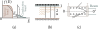
\includegraphics[scale=1.1]{figures/ch_08/fig_8_25.pdf}
		\caption[]{(a)---electron distribution plots for equilibrium (solid line) and inverse (dotted line) states of semiconductor; (b)---development of photon avalanche caused by induced radiation of a quantum system with population inversion; (c)---in a quantum generator only the radiation which propagates along the $00'$ axis is amplified.}
		\label{fig:8_25}
	\end{center}
	\vspace{-0.8cm}
\end{figure}

There are various methods of creating a population inversion of the semiconductor energy bands. The best prospects offers the minority carrier injection through a forward biased p-n junction made in a degenerate semiconductor. Figure \ref{fig:8_26} shows the structure of a semiconductor laser in which such method of pumping is used. The laser is a diode with a p-n junction $1$ made in the form of a bar. Highly polished faces $2$ of this bar made strictly parallel to each other play the part of mirrors that reflect the photons.

The interest for the semiconductor lasers is due to some of their remarkable properties.

First of all, they have a high efficiency which may in principle reach $100\%$. This is due, on the one hand, to the quantum mechanical nature of the laser as a system in which only the ``working'' energy levels are excited, and on the other, to the fact that in a semiconductor laser, the electric energy is directly converted into coherent radiation without any intermediate steps as in all the other laser types.

Another remarkable property of the semiconductor laser is that it is possible to modulate the coherent radiation directly by changing the current through the p-n junction. This enables them to be used in communications and in television as well as in ultra-high-speed computers for which their miniature dimensions are of special importance.

\begin{figure}[t]
	\begin{center}
		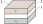
\includegraphics[scale=1.1]{figures/ch_08/fig_8_26.pdf}
		\caption[]{Schematic representation of semiconductor laser: $1$---active region of laser; $2$---reflecting faces (mirrors).}
		\label{fig:8_26}
	\end{center}
	\vspace{-0.8cm}
\end{figure}

\section{Fundamentals of integrated circuit electronics (microelectronics)}\label{sec:78}

The progress of modern science and technology requires electronics to provide for it efficient complex electronic equipment. Such equipment often contains hundreds of thousands of elements connected
into a circuit by means of a similar number of connections.

Electronic equipment is responsible for the main part of costs of production of modern military equipment and aircraft. According to Western sources, the cost of electronic equipment makes up over $70\%$ of the cost of a modern guided missile and over $50\%$ of the cost of a modern bomber.

To produce such highly sophisticated equipment some difficult problems had to be solved, including the problems of drastic reduction in weight, dimensions, power consumption, and in price and of increasing the reliability of electronic devices.

Should modern electronic apparatus be assembled from components manufactured by the industry several decades ago, its weight would have been tons, its dimensions cubic metres, and its power consumption hundreds of kilowatts. The latter fact would have sufficed to make it impractical for many fields of the economy.

But those are not the only drawbacks. As the complexity of the electronic equipment increases its reliability---a factor of primary importance especially in military, computer and automatic production line applications---diminishes.

Finally, the problem of bringing down the costs of electronic equipment is also not devoid of importance and this problem can only be solved by far-reaching automation of the technological processes, which in turn requires the development of appropriate technology.

The efforts to solve those problems, lead to the creation of miniature electronic elements and blocks based on solid-state technology and to the microminiaturization of electronic equipment, resulting finally in the birth of a new field of modern electronics---microelectronics---whose main objective is the production of highly reliable and economical microminiature electronic circuits and apparatus.

The modern way to solve this problem is to devise new principles of constructing electronic circuitry, which would make possible the formation of a circuit as a whole on a miniature semiconductor crystal instead of assembling it from separate components. Such solid electronic circuits designed for specific applications are termed \textit{integrated circuits} (IC). The integrated circuit, like an ordinary electronic circuit, is made up of active elements (transistors, diodes) and of passive elements (capacitors and resistors).

A semiconductor IC is fabricated on a single-crystal wafer (usually silicon) with the aid of methods of local doping with appropriate impurities to produce on it transistors, diodes, capacitors, and resistors and to connect them into a circuit. The dimensions of the wafer are typically $\parenthesis{\num{e-2}}\times\parenthesis{\num{5e-3})}times\parenthesis{\num{2e-4}}$ \si{\metre\cubed}, the area of the active elements, for instance of a transistor, being under \SI{e-9}{\metre\squared}.

The integrated circuits are usually characterized by packing density and by degree of integration. The packing density is the number of elements per unit volume of the IC, and the degree of integration, the number of elements making up the IC. Table \ref{table:8_2} presents data on the packing density and on failure rate of circuits of different generations.

\begin{table}[!b]
	\renewcommand{\arraystretch}{1.2}
	\caption{}
	\vspace{-0.6cm}
	\label{table:8_2}
	\begin{center}\resizebox{0.98\linewidth}{!}{
			\begin{tabular}{lcc}
				\toprule[1pt]
                \textbf{Circuits using} & \textbf{Number of elements per} \si{\metre\cubed} & \textbf{Failure rate}, $\lambda$ (\si{\per\hour})\\
                \midrule[0.5pt]\midrule[0.5pt]
                Pre-1941 elements & \num{3.5e4} & \num{e-5}\\
				Miniature elements & \num{1.8e5} & \num{5e-6}\\
				Semiconductor IC & \num{3.0e9} & Negligible\\
				\bottomrule[1pt]
			\end{tabular}
	}\end{center}
\end{table}

It follows then that, the changeover from the circuits assembled from pre-1941 components to modern IC increased the packing density some \num{e5} times. There are reports of packing densities of IC of up to \SI{e15}{\per\metre\cubed}.

The degree of integration of an IC may vary in a wide range---from tens to hundreds or thousands of elements on each wafer. IC of over $100$ elements are termed \textit{big integrated circuits} (BIC).

The power consumption of IC, depending on the type, lies in the range of hundreds of milliwatts to several microwatts.

Thus, the changeover to electronic equipment designed around IC practically solved the problems of dimensions, weight, and power consumption. Electronic computers are an impressive example of this. The first Soviet computers which were assembled from vacuum tubes and radio components (Minsk, Ural, etc.) occupied whole buildings, weighed tons, and consumed tens of kilowatts of power.

Electronic blocks assembled from IC have dimensions of the order of \SI{e-2}{\metre\cubed} and consume only hundreds of watts while special computers used, for instance, for launching and controlling missiles and spacecraft have dimensions of the order of \SI{e-3}{\metre\cubed}, weigh tens of kilograms and consume power of the order of tens of watts.

Presently BIC are being used in single wafer electronic calculators. The computer wafer (called ``chip'') of such a device is $(5\times 5)\SI{e-6}{\metre\squared}$ and contains about $5000$ transistors. BIC for electronic time-pieces including wrist watches have been developed as well. In such watches two wafers containing about $2000$ transistors are used.

A substantial advantage of IC is that because mass-produced IC are much cheaper than equivalent circuits assembled from components. Modern technology makes it possible to arrange about a thousand IC on one single-crystal wafer of $\SI{5e-2}{\metre}$ in diameter; if a hundred such wafers are processed at a time, about a million IC can be produced in one technological cycle.

The progress in microelectronics is a very rapid one. During the last decade a distance was covered from the simplest IC to BIC. In the nearest future, it is expected that most electronic equipment shall be based on integrated circuitry with the degree of integration increasing $100$ to $1000$-fold and a much greater reliability being attained. However, there are obstacles on this road, namely the so-called ``tyranny of numbers'' of microelements which already today crowd complex equipment in tens or hundreds of millions. To overcome this obstacle, it will, probably, be necessary to change over from the conventional IC to functional circuits, that is, to devices designed for specific functions and operating on some specific principle of solid state physics as a whole and not as a sum of individual elements (transistors, diodes, etc.).

As the simplest example of a functional device one may cite the ac-dc converter. The conventional circuit of such a converter consists of a transformer, rectifiers (semiconductor or vacuum diodes), and a filter. The functional converter consists of a resistance region in which the ac energy is transformed into heat, of the central low electric but high heat conductivity region, and of a thermoelectric region in which heat is converted into dc power. In such a device it is impossible to separate regions equivalent to the components of a conventional circuit. Here, the crystal as a whole fulfills the complex function of an ac-dc converter.

The transition to functional circuits should result in a drastic decrease in the number of components and, therefore, in the decrease in the cost and in dimensions and in the improvement of reliability.

The process of creation of new scientific and technological trends in electronics and of devising devices and equipment based on new principles is a continuous one, the foundation for it being the utilization of the top-ranking achievements in the fundamental and applied sciences, first of all, in physics. Here, the leading role belongs to solid state physics which determines the mainstream of progress in modern electronics.
